
\documentclass[11pt,letterpaper]{article}

% Load some basic packages that are useful to have
% and that should be part of any LaTeX installation.
%
% be able to include figures
\usepackage{graphicx}
% get nice colors
\usepackage{xcolor}

% change default font to Palatino (looks nicer!)
\usepackage[latin1]{inputenc}
\usepackage{mathpazo}
\usepackage[T1]{fontenc}
% load some useful math symbols/fonts
\usepackage{latexsym,amsfonts,amsmath,amssymb}

% comfort package to easily set margins
\usepackage[top=1in, bottom=1in, left=1in, right=1in]{geometry}

% control some spacings
%
% spacing after a paragraph
\setlength{\parskip}{.15cm}
% indentation at the top of a new paragraph
\setlength{\parindent}{0.0cm}


\begin{document}

\begin{center}
\Large
Ay190 -- Worksheet 16\\
Anthony Alvarez\\
Date: March 11, 2014
\end{center}

\section{Finite Volume Shock}

We implement a Finite Volume Code for a Shock Tube with the following parameters on a 
domain of $[-0.5,0.5]$ with
$r= 0$, $\rho_L = 1.0$, $\epsilon_L = 2.5$, $v_L = 0$, and on the right side
$\rho_R = 0.25$, $\epsilon_R = 1.795$, $v_R= 0$ and the adiabatic exponent of 
$\gamma = 1.4$ .

\subsection{Commpare Methods}

We implement the code in python and run it to a final time of $t = 0.2$. 

For the various methods (piecewise constant, TVD-midmod, and TVDMC2) we record
the amount of time it takes to compute $0.2$ seconds worth of simulation. We get
$38.21$ , $50.53$, $63.93$, seconds for the three methods respectively, with out
any graphing.

At the final time of $t=0.2$ we can see in  ~\ref{fig:0} that the 
shock has completely devloped but is missing features near the initial 
discontiuity. The rarefraction has compeletly eclipsed the nearest density
plateau.

\begin{figure}[bth]
\centering
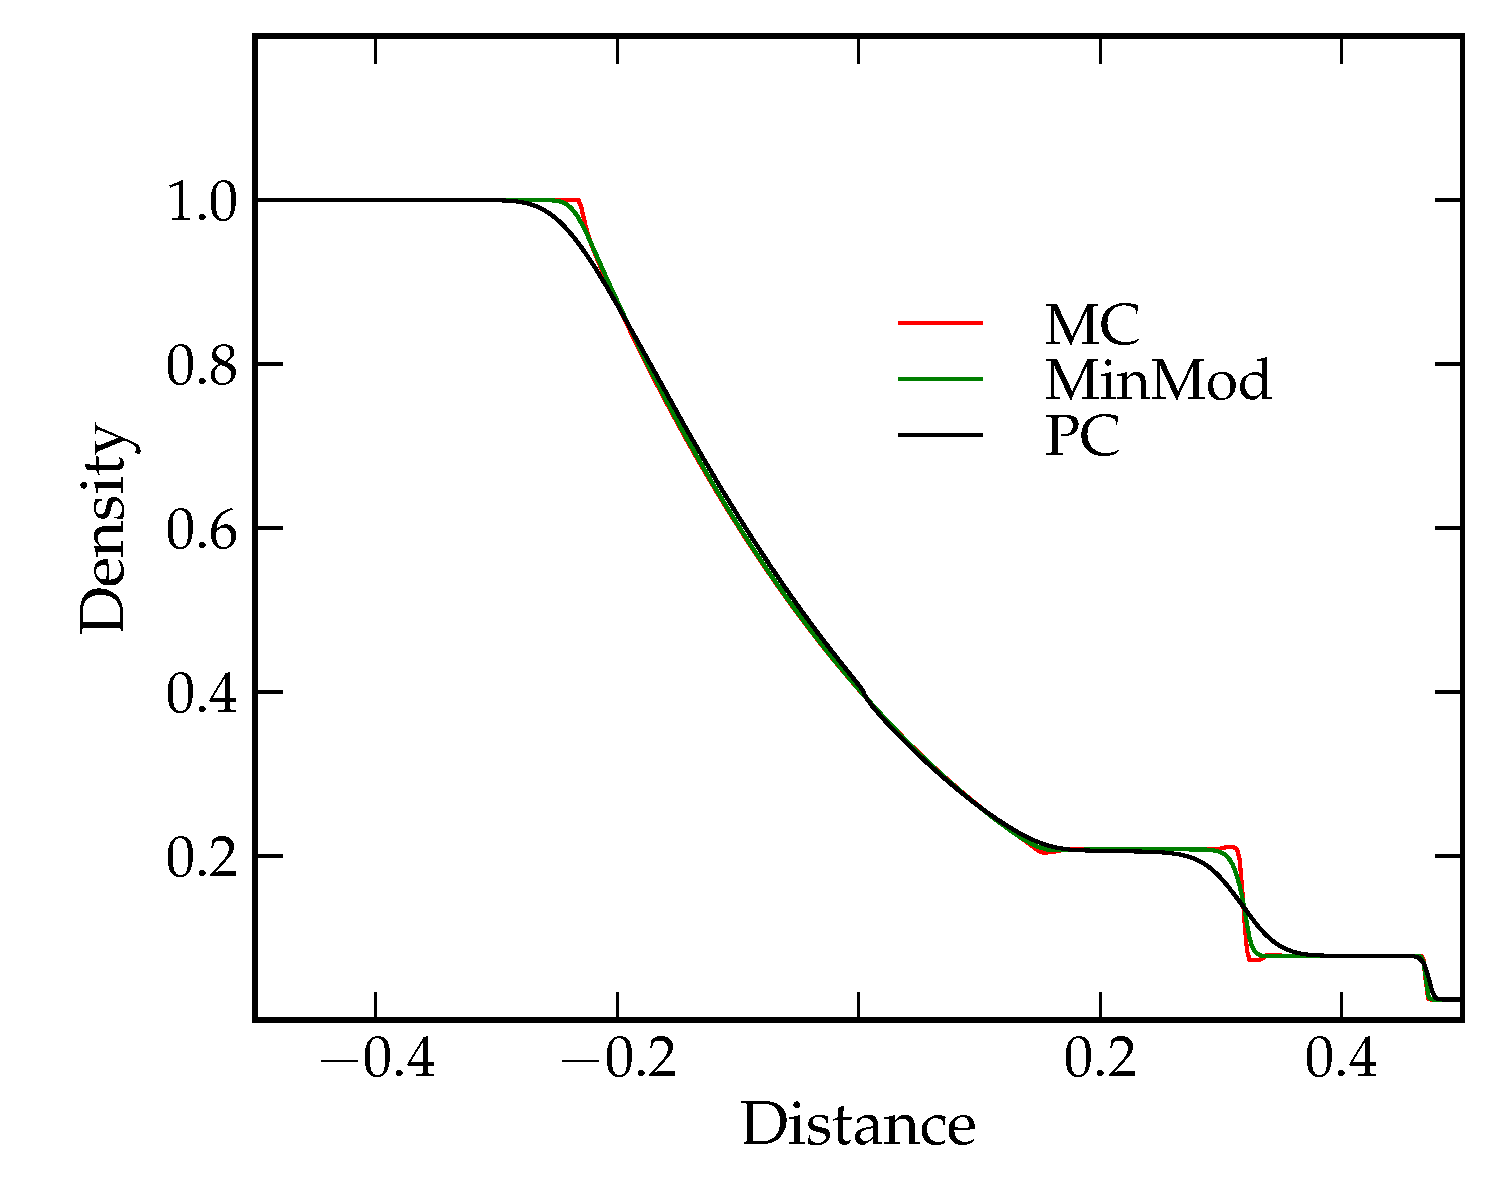
\includegraphics[width=0.5\textwidth]{Compare Finite Volume.pdf}
\caption{Graph of density with respect to space on the domain 
$[-0.5,0.5]$. At time $t = 0.2$ for three different methods.}
\label{fig:0}
\end{figure}

\subsection{Compare to SPH and Exact Solution}

The Finite Volume Hydro code we've implemented seems to differ greatly from the
exact solution. The finite volume codes have expanded the rarefraction and
completely obliterated the first plateau at roughly $x=0$, while the SPH sill 
maintains this feature. ~\ref{fig:compare} Note that we have the same number
of grid points as particles, $n = 500$.

\begin{figure}[bth]
\centering
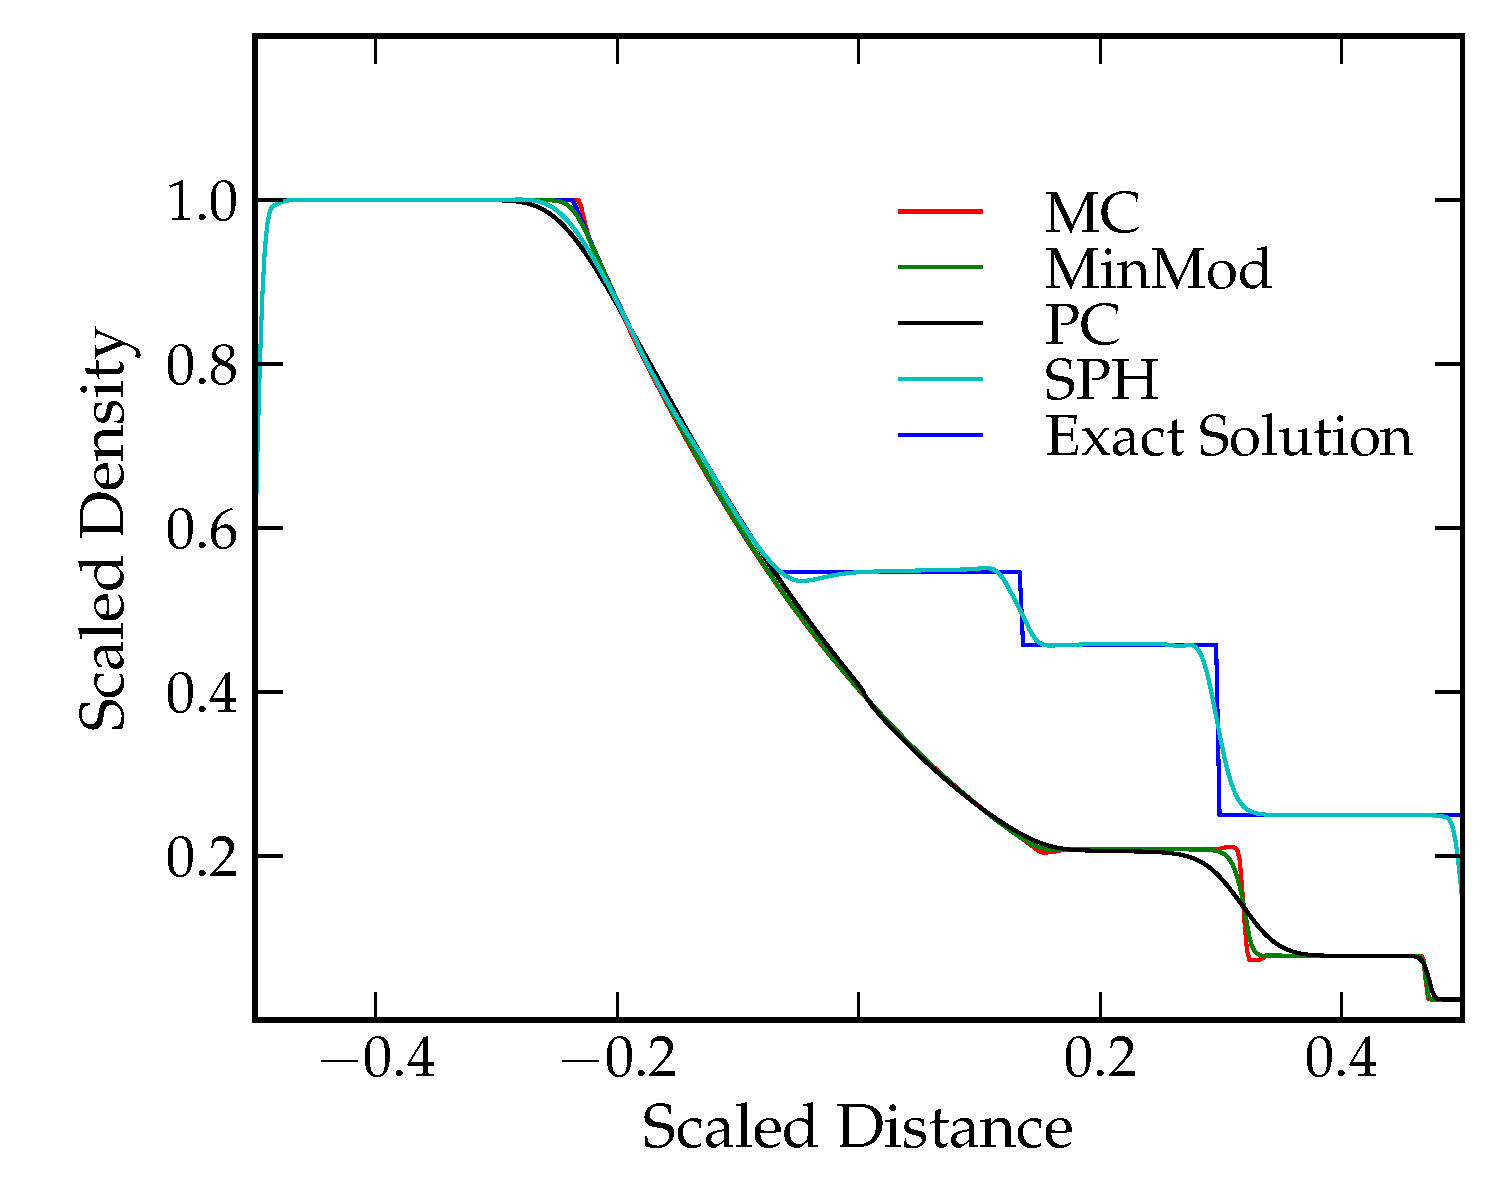
\includegraphics[width=0.5\textwidth]{compare.pdf}
\caption{Graph of density with respect to space on the domain 
$[-0.5,0.5]$. At time $t = 0.2$ for three different methods.}
\label{fig:compare}
\end{figure}

\subsection{Code Improvements} 

Our finite volume code initially used slow for loops making the code take
upwards of a minute to simulate to $t = 0.2$. By leveraging numpy array
operations we are greatly able to reduce the runtime. For the methods 
piecewise constant, TVD-midmod, and TVD-MC2 we are able to get computation times
of $4.08$, $7.07$, $7.86$ seconds without any graphing. We get a $9$ times speed
up on piecewise constant, $7$ times speed up on midmod, and an $8$ times speed up
on mc2. This is a huge improvement from just a few changes to the code. You can
see the array based implementation in hydro\_1D\_FV.py while the loop 
implementation can be found in hydro\_1D\_FV.py.


\end{document}

